%\usepackage{cleveref}
\chapter{Results \& Conclusions}

\label{ch:results}

\section{ATLAS\textsuperscript{3D}}
Initially, the algorithm was trained using the $\lambda_{Re}$ to predict the FS classification since they were related directly. Promisingly, the classifier was 100\% successful in its predictions. Training was then performed using the Se\'rsic index of the single fit, n, and achieved success of 71\%.
\begin{figure}[h!]
	\centering
	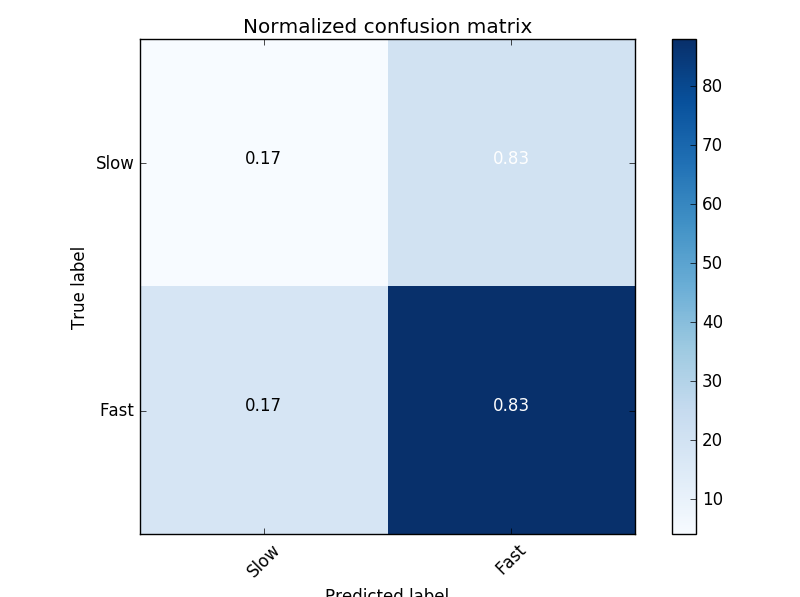
\includegraphics[width=\textwidth]{norm_conf_mat_Sersic_normalised.png}
	\caption{Confusion Matric for predictions based on Se\'rsic Index.
	}
	\label{fig:confmatDT}
\end{figure}
We can estimate how the model succeeded for the separate populations compared to that predicted by the binomial probability distribution which is necessary due to the binomial nature of the outcome with differing sizes of the two populations, given by\cite{simmons_2016}:
\begin{equation}
P(k,n) = \binom{n}{k}p^{k}q^{n-k}
\end{equation}
where $n$ is the number of trials, $k$ is the number of successes, $n-k$ is the number of failures, $p$ is the probability of success in one trial and $q=1-p$ is probability of failure in one trial. Since the binomial distribution does not take account of the order of the successes, we adapt the binomial formula by removing the permutations factor:
\begin{equation}
P(k,n) = p^{k}q^{n-k}
\end{equation}
By treating the 2 populations separately we can therefore define success as a correct classification, and the probabilities are given by the overall relative number proportions of the 2 populations, i.e.,
\begin{equation}
P_{f}(k_{f},n_{f}) = p_{f}^{k_{f}}q_{f}^{n_{f}-k_{f}}
\end{equation}
and,
\begin{equation}
P_{s}(k_{s},n_{s}) = p_{s}^{k_{s}}q_{s}^{n_{s}-k_{s}}
\end{equation}
where the subscripts denote the 2 populations.This gives a $\approx$ 2\% probability of producing these results based on a random guess for slow rotators and a negligible probability for fast rotators, suggesting a significant improvement. \\
When we look at the D/T dependence of the $\lambda_{Re}$ value, we see a more promising separation of the two populations, with a value of D/T $\approx 0.28$ producing a low level of impurity. This parameter was identified as the most promising by \cite{Krajnovic2013}.
\begin{figure}[ht]
	\centering
	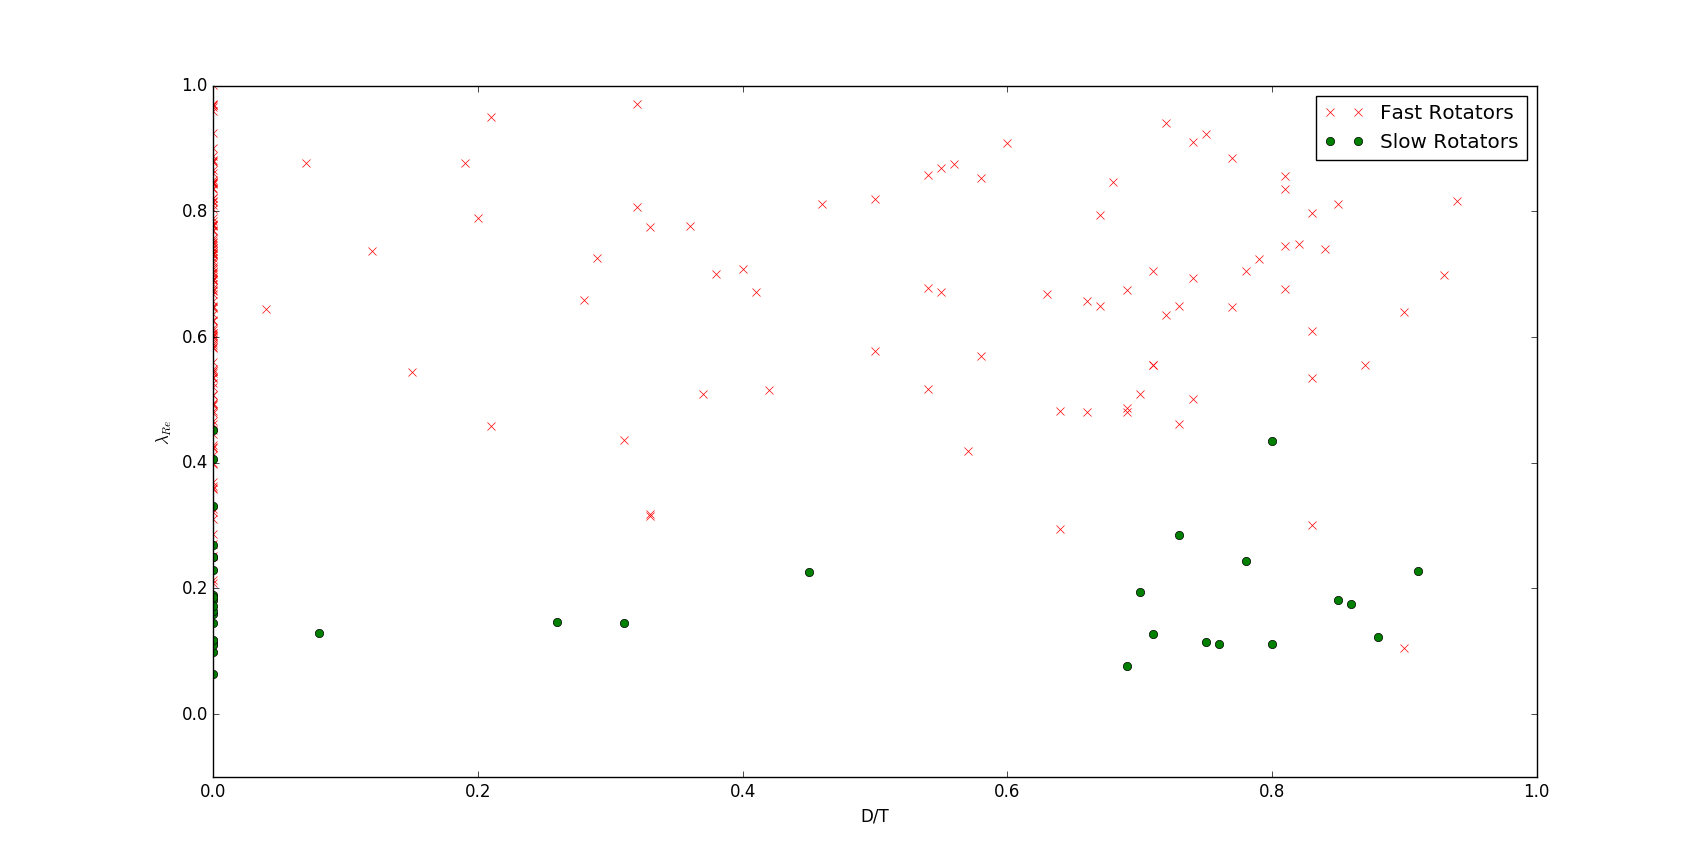
\includegraphics[width=\textwidth]{DT_lamre.png}
	\caption{The separation between the two populations is more pronounced here. The galaxies with D/T = 0 have no exponential discs.
	}
	\label{fig:dtlamre}
\end{figure}
The algorithm was then trained using D/T, improving the success rate to 81\%. Interestingly, when we evaluate the success of the decision tree classifier for those galaxies with no exponential disk component, where D/T$\lesssim $0.05, we find that the decision tree is still able to correctly classify the majority of galaxies.
\begin{figure}[h!]
	\centering
	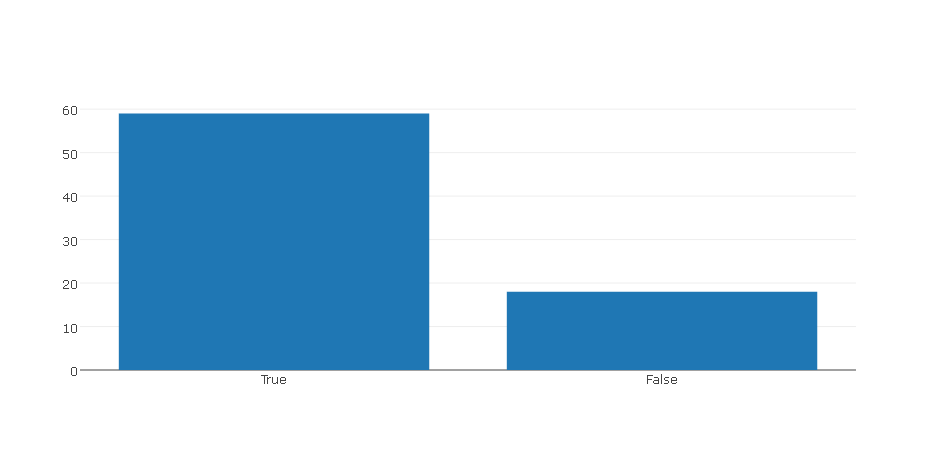
\includegraphics[width=\textwidth]{DTSuccessBar.png}
	\caption{Prediction success for galaxies with D/T $\lesssim$ 0.05.}
	\label{fig:dtbar}
\end{figure}
\begin{figure}[h!]
	\centering
	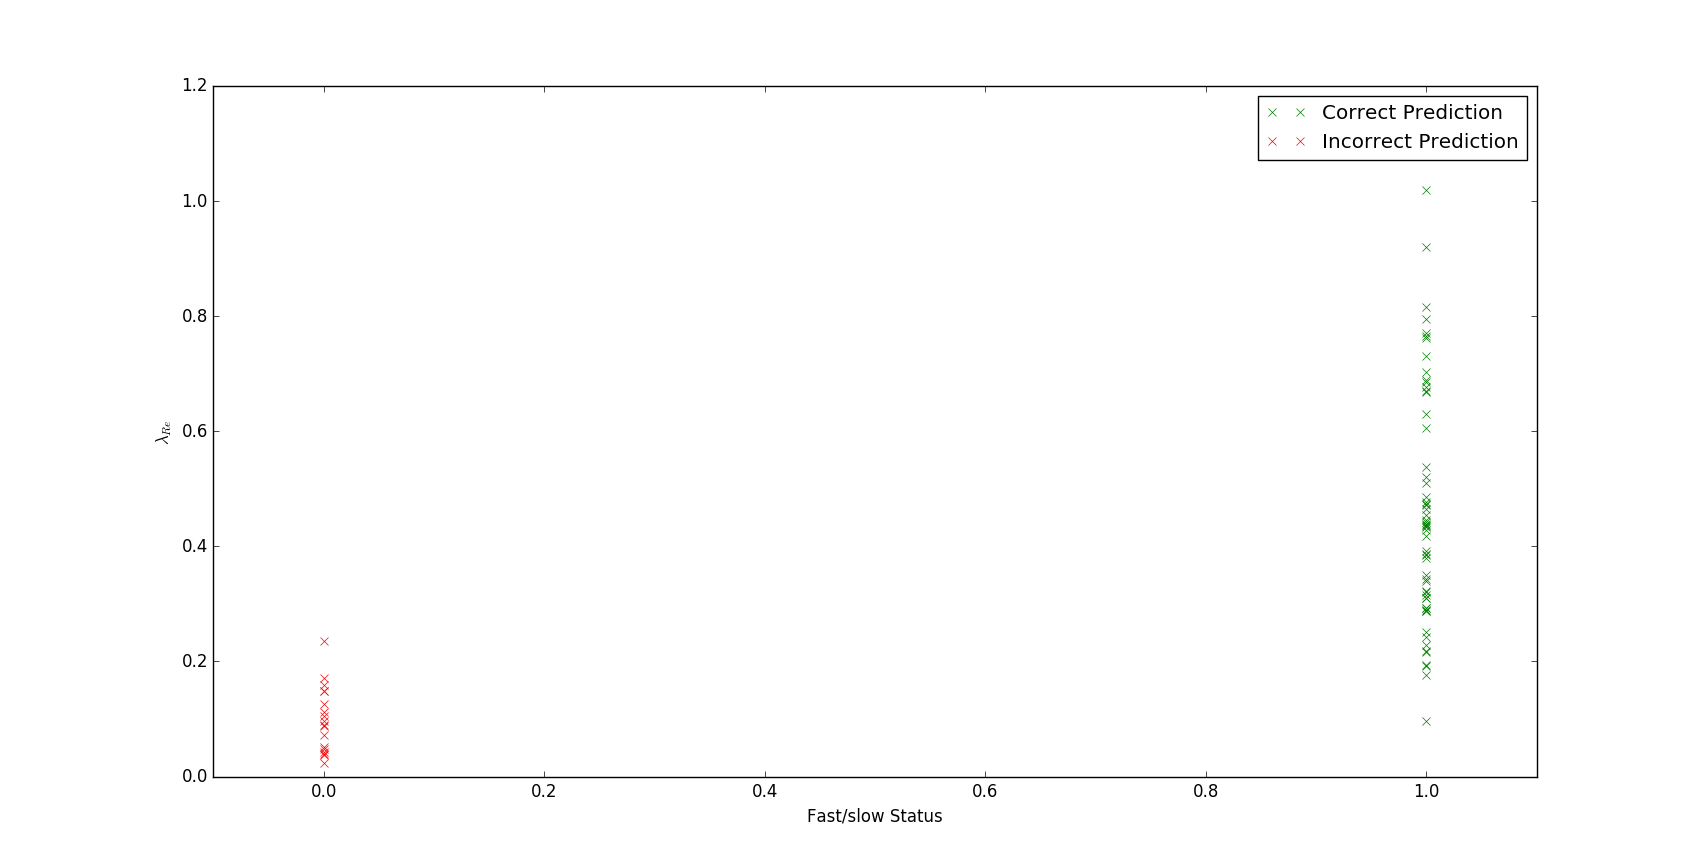
\includegraphics[width=\textwidth]{zerodt.png}
	\caption{Investigating the results where D/T$\lesssim $0.05. We see that the algorithm predicts galaxies to be universally fast rotators.
	}
	\label{fig:zerodt}
\end{figure}
The success rate for just these galaxies is $\approx$77\% which is more than that expected from the binomial distribution. However, the apparent success is undermined when we plot the results for just these galaxies in \ref{fig:zerodt}.
The algorithm benefited from the fact that only $\approx$10\% of the galaxies with no disk in the test set were slow rotators. If the choice was made randomly, the success would be $\approx$15\%, and so represents a significant improvement, but would hardly require such statistical learning methods to make the conclusion that if there is no disk it is most likely a fast rotator.
The algorithm was then trained using both D/T and Se\'rsic index of the single fit by passing the features as an $n\times 2$ matrix, resulting in a success rate of 75\%, exceeding expectations based on random guess alone slightly, but is less than what was achieved using D/T alone. 
\begin{figure}[h!]
	\centering
	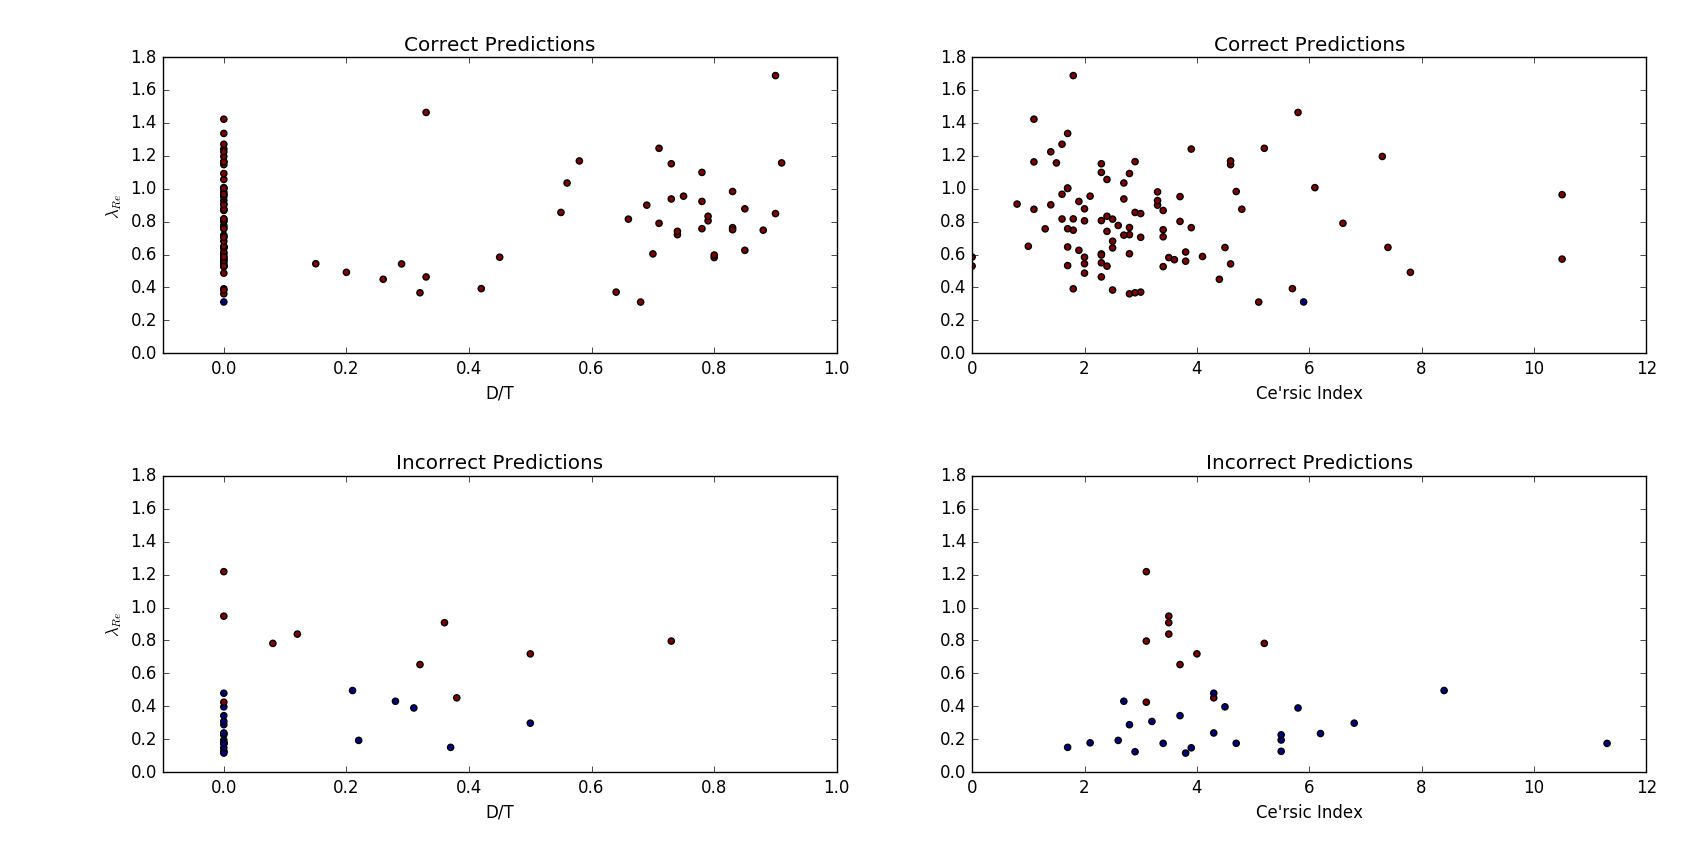
\includegraphics[width=\textwidth]{multiplot_correctincorrect_2d_withcol.png}
	\caption{Evaluating the success of decision trees with 2 variables, se\'rsic index and D/T. The markers are colour coded to be magenta for fast rotators and blue for slow rotators.
	}
	\label{fig:correctvsincorrect}
\end{figure}
\begin{figure}[h!]
	\centering
	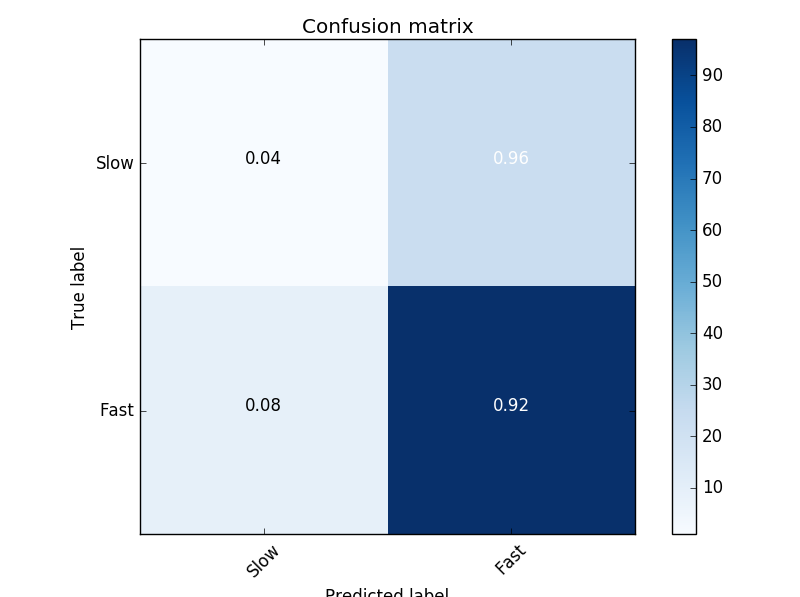
\includegraphics[width=\textwidth]{norm_conf_mat_DTandSersic_normalised.png}
	\caption{Confusion Matric for predictions based on D/T and Se\'rsic Index.
	}
	\label{fig:confmatDT}
\end{figure}
The plots \ref{fig:correctvsincorrect} and \ref{fig:confmatDT} suggest that the algorithm is predicting slow rotators slightly more often rather than blindly assuming all galaxies are fast rotators, but it only successfully predicts a slow rotator once.
These results suggest that the use of decision trees with parameters initialised to their defaults are not very promising. However, there are a large number of parameters, as outlined in the preceding sections, that can be tuned to maximise the efficiency of the classifier. SKlearn has the inbuilt function GridSearchCV that performs an exhaustive search over specified parameter values for an estimator. To avoid difficulties posed by a limited dataset size, the algorithm uses a k-fold cross-validation where:
\begin{quotation}
	The original sample is randomly partitioned into k equal size subsamples. Of the k subsamples, a single subsample is retained as the validation data for testing the model, and the remaining k-1 subsamples are used as training data. The cross-validation process is then repeated k times (the folds), with each of the k subsamples used exactly once as the validation data. The k results from the folds can then be averaged (or otherwise combined) to produce a single estimation. The advantage of this method is that all observations are used for both training and validation, and each observation is used for validation exactly once.\cite{vanschoren}
\end{quotation}
This was performed using the possible options:
\begin{itemize}
	\item criterion:['gini','entropy']
	\item splitter:['best','random']
	\item max\_features:['sqrt','log2',None]
	\item max\_depth:range(1,10)
\end{itemize}
In so doing, the success rate was increased to $\approx$ 93\%, with the following options:
\begin{itemize}
	\item criterion='entropy'
	\item splitter='best'
	\item max\_features='sqrt'
	\item max\_depth=4
\end{itemize}
In conclusion, decision trees offer promising results in identifying fast from slow rotating galaxies but requires some initial sorting of the data and careful model selection. The presence of a large number of galaxies with no disk component significantly skewed the results, and would best be initially filtered out since no new information is to be gained from their inclusion. Further study would focus on galaxies that have no disk component exclusively to see if better results can be achieved.